## Recursividad: Conejitos cariñosos {.fragile}

\setbeamertemplate{itemize/enumerate body begin}{\footnotesize}
\setbeamertemplate{itemize/enumerate subbody begin}{\footnotesize}

\vspace{-2ex}

- Mes 0: De una casa se escapa una pareja de conejos bebés.
- Mes 1: Estos conejos, al mes ya son adultos.
- Mes 2: Ya tienen un par de crías.
    - Son de una raza que siempre paren un macho y una hembra.
- Mes 3: La pareja original tiene otro par de crías.
    - La primera pareja de hijos ya es adulta.
- Mes 4: La pareja original de nuevo tiene otro par de crías.
    - La primera pareja de hijos también aporta con un par de crías.
    - La segunda pareja de hijos ya es adulta.
- Mes 5: La pareja original de nuevo tiene otro par de crías.
    - La primera pareja de hijos tiene su segundo par de crías.
    - La segunda pareja de hijos pare por primera vez.
    - La tercera pareja de hijos ya es adulta.
- Así, sucesivamente...

\bgnblocknormal
¿Cuántas parejas de conejos hay en el mes \bld{n}?
\trmblocknormal

\placeLogo{img/rabbit-1f407.pdf}

## Recursividad: Conejitos cariñosos {.fragile}

\newcommand{\nzRbbS}{
\includegraphics[width=9mm]{img/twoRabbits.pdf}}
\newcommand{\nzRbbX}{
\includegraphics[width=12mm]{img/twoRabbits.pdf}}
\tikzset{
  % style for inserting images as nodes
  img/.style={
    % text width=8mm,
    minimum height=4mm,
    anchor=center,
    %text height=2cm,                 %% don't use this
    inner sep=0pt,     %% use this
    outer sep=0pt,     %% and this
    % rectangle,
    % align=center,
    % draw,thick % only for debugging..
  },
  treeLines/.style={
    ultra thick, black
  },
}
\begin{tikzpicture}

  \matrix (rbbs) [matrix of nodes, nodes=img, row sep=4mm, column sep=0mm]{
   \footnotesize{Mes}    &         &         &         &         &         &         &        &        & \footnotesize{Parejas} \\
   0 &         &         &         &         & \nzRbbS &         &         &         & 1      \\
   1 &         &         &         &         & \nzRbbX &         &         &         & 1      \\
   2 &         & \nzRbbS &         &         & \nzRbbX &         &         &         & 2      \\
   3 &         & \nzRbbX &         &         & \nzRbbX &         & \nzRbbS &         & 3      \\
   4 & \nzRbbS & \nzRbbX &         & \nzRbbS & \nzRbbX &         & \nzRbbX &         & 5      \\
   5 & \nzRbbX & \nzRbbX & \nzRbbS & \nzRbbX & \nzRbbX & \nzRbbS & \nzRbbX & \nzRbbS & 8      \\
  };

% parejas
\draw[treeLines] (rbbs-2-6) -- (rbbs-3-6);
\draw[treeLines] (rbbs-3-6) -- (rbbs-4-6);
\draw[treeLines] (rbbs-4-6) -- (rbbs-5-6);
\draw[treeLines] (rbbs-5-6) -- (rbbs-6-6);
\draw[treeLines] (rbbs-6-6) -- (rbbs-7-6);
% parejas
\draw[treeLines] (rbbs-4-3) -- (rbbs-5-3);
\draw[treeLines] (rbbs-5-3) -- (rbbs-6-3);
\draw[treeLines] (rbbs-6-3) -- (rbbs-7-3);
% parejas
\draw[treeLines] (rbbs-5-8) -- (rbbs-6-8);
\draw[treeLines] (rbbs-6-8) -- (rbbs-7-8);
% parejas
\draw[treeLines] (rbbs-6-2) -- (rbbs-7-2);
% parejas
\draw[treeLines] (rbbs-6-5) -- (rbbs-7-5);

% hijos
\draw[treeLines] (rbbs-3-6) -- (rbbs-4-3);
\draw[treeLines] (rbbs-4-6) -- (rbbs-5-8);
\draw[treeLines] (rbbs-5-3) -- (rbbs-6-2);
\draw[treeLines] (rbbs-5-6) -- (rbbs-6-5);
\draw[treeLines] (rbbs-6-3) -- (rbbs-7-4);
\draw[treeLines] (rbbs-6-6) -- (rbbs-7-7);
\draw[treeLines] (rbbs-6-8) -- (rbbs-7-9);

\end{tikzpicture}

## Recursividad: Sucesión de Fibonacci {.fragile}

\bgnblocknormal
\bld{La sucesión de Fibonacci} se define recursivamente como:
\trmblocknormal

\vspace{-2ex}

$$ F_n = \begin{cases}
        n                 & \;\;\;\;\text{si} \;\;\;\; 0 \leq n \leq 1 \\
        F_{n-1} + F_{n-2} & \;\;\;\;\text{si} \;\;\;\; n > 1 \\
    \end{cases}
$$

\vspace{1ex}
\begin{lstlisting}[style=frame02]
# fibonacci: int -> int
# Calcula el n-ésimo valor de la sucesión de Fibonacci.
# Ejemplo: fibonacci(8) retorna 21
def fibonacci(n):
    if n <= 1:            # caso base
        return n
    else:                 # caso recursivo
        return fibonacci(n - 1) + fibonacci(n - 2)
# Tests
assert fibonacci(0) == 0
assert fibonacci(9) == 34
\end{lstlisting}

## Recursividad: Sucesión de Fibonacci {.fragile}

\bgncolumns
\column{.45\textwidth}

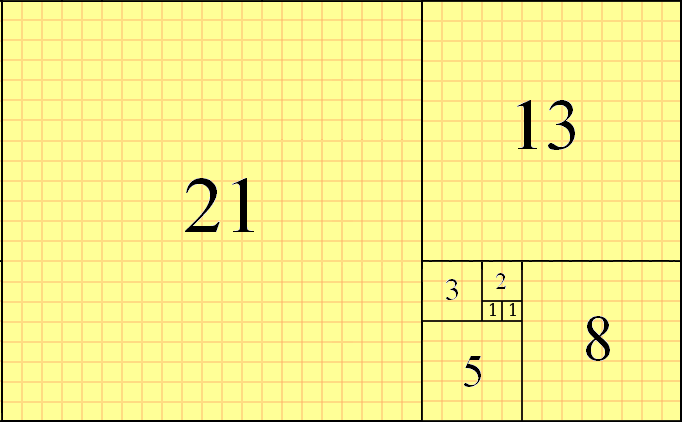
\includegraphics[width=\textwidth]{img/FibonacciBlocks.png}

\footnotesize{https://commons.wikimedia.org/
wiki/File:34*21-FibonacciBlocks.png}
\column{.1\textwidth}
\column{.45\textwidth}

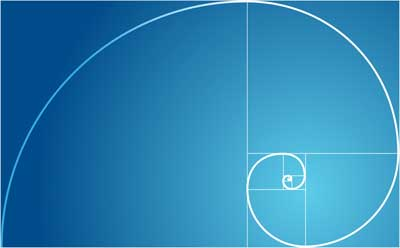
\includegraphics[width=\textwidth]{img/fibonacci-nature-3.jpg}

\footnotesize{iStockphoto.com/Janne Ahvo}

\trmcolumns

## Recursividad: Series {.fragile}

\bgnblockgood
\strongText{Ejemplo 6:} Determine la suma de: $1 + 2 + 3 + 4 + \ldots + n$.
\trmblockgood

\pause

\begin{lstlisting}[style=frame02]
# suma1n: int -> int
# Calcula la suma de los primeros n números naturales.
# Ejemplo: suma1n(3) retorna 6
def suma1n(n):
    if n == 1:
        return 1
    else:
        return n + suma1n(n - 1)
# Tests
assert suma1n(1) == 1
assert suma1n(6) == 21
\end{lstlisting}

## Recursividad: Series {.fragile}

\bgnblockgood
\strongText{Ejemplo 7:} Calcule el valor de: $\quad\sum\limits_{0}^n \frac{1}{2^n}$
\trmblockgood

\pause

\begin{small}
\begin{lstlisting}[style=frame02]
# unMedioCeroN: int -> num
# Calcula el valor de la serie cuyo término enésimo es 1/(2^n),
# partiendo desde 0.
# Ejemplo: unMedioCeroN(5) retorna 1.96875
def unMedioCeroN(n):
    if n == 0:
        return 1
    else:
        return (1 / (2.0**n)) + unMedioCeroN(n - 1)
# Tests
assert unMedioCeroN(1) == 1.5
assert unMedioCeroN(6) == 1.984375
\end{lstlisting}
\end{small}

## Recursividad: Series {.fragile}

\bgnblockgood
\strongText{Ejemplo 8:} Calcule el valor de: $\quad\sum\limits_{1}^n \frac{1}{2^n}$
\trmblockgood

\pause

\begin{small}
\begin{lstlisting}[style=frame02]
# unMedioUnoN: int -> num
# Calcula el valor de la serie
# cuyo término enésimo es 1/(2^n),
# partiendo desde 1.
# Ejemplo: unMedioUnoN(5) retorna 0.96875
def unMedioUnoN(n):
    if n == 1:
        return 1/2.0(*@\tikzmark{markBgnHalf}@*)
    else:
        return (1 / (2.0**n)) + unMedioUnoN(n - 1)
# Tests
assert unMedioUnoN(1) == 0.5
assert unMedioUnoN(6) == 0.984375
\end{lstlisting}
\end{small}

\drawTikZComment[above right=-0.2em and 7em of markBgnHalf, text width=10em]{markBgnHalf}{\scriptsize Ojo, acá el primer valor es $\mathbf{\frac{1}{2}}$}

## Recursividad: Torres de Hanói {.fragile}

- Es un puzzle/juego matemático.
- Consiste en varios discos de distinto tamaño y tres torres.
- La idea es que todos los discos, que inicialmente están en la torre
izquierda, hay que moverlos hasta la torre derecha, respetando las siguientes reglas:
    1. Sólo un disco puede ser movido cada vez.
    1. Un disco sólo puede ser movido sobre una torre vacía o sobre otro disco más grande.

\centering    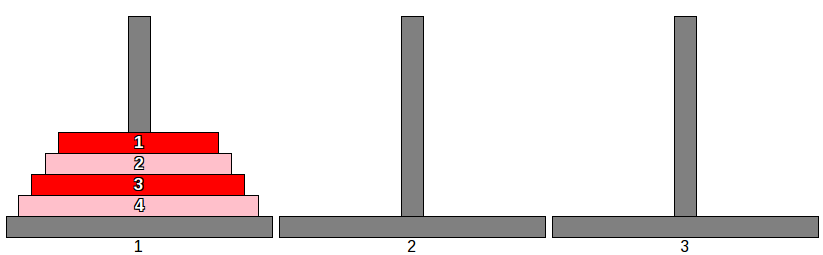
\includegraphics[width=.8\textwidth]{img/towersHanoi.png}

## Recursividad: Torres de Hanói {.fragile}

- Nuestro objetivo es saber cuántos son los pasos mínimos para resolver el juego, dados
$n$ discos.
- También se quiere determinar la mejor secuencia de pasos para resolverlo.

- Se puede ver una demostración interactiva en: \url{https://nozimica.github.io/hanoi/}


